
% Age of Aquarius chapter =============================================
\chapter*{Age of Aquarius}
\addcontentsline{toc}{chapter}{Age of Aquarius}

\begin{flushright}
\parbox{0.8\textwidth}{
\emph{The greatest difficulty with the world is not its ability to produce, but the unwillingness to share. \\
\hspace*{\fill}{\textperiodcentered \textperiodcentered \textperiodcentered \hspace*{0.2em} Roy L. Smith} } }
\end{flushright}

\noindent
Age of Aquarius is chess variant which is played on 14 x 14 board,
with light yellow and light green fields and light tan-gold and
dark green pieces. In algebraic notation, columns are enumerated
from 'a' to 'n', and rows are enumerated from '1' to '14'. A new
piece is introduced, Unicorn.

\clearpage % ..........................................................
% Unicorn *************************************************************

\section*{Unicorn}
\addcontentsline{toc}{section}{Unicorn}

\noindent
\begin{wrapfigure}[5]{l}{0.4\textwidth}
\centering
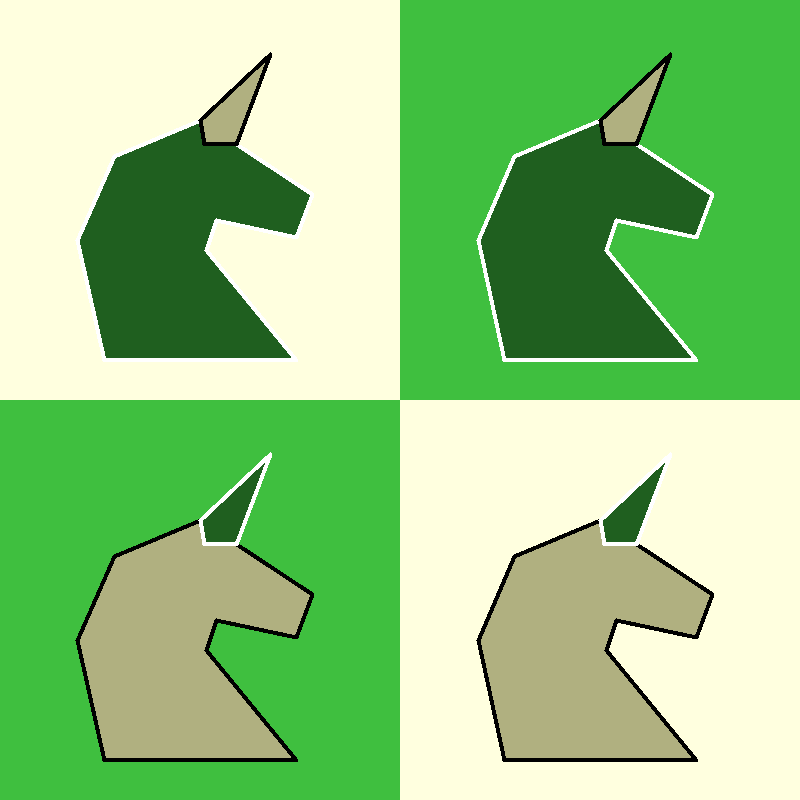
\includegraphics[width=0.4\textwidth, keepaspectratio=true]{pieces/09_unicorn.png}
\caption{Unicorn}
\label{fig:09_unicorn}
\end{wrapfigure}
Unicorn is a piece similar to Knight, only it can jump longer on
opposite color fields. Just as Knight, Unicorn is not obstructed
by any piece in its' surroundings.

\vspace{7\baselineskip}
\subsection*{Movement}
\addcontentsline{toc}{subsection}{Movement}

\noindent
\begin{wrapfigure}{l}{0.4\textwidth}
\centering
\includegraphics[width=0.4\textwidth, keepaspectratio=true]{examples/08_aoa/scn_aoa_01_unicorn_same_color.png}
\caption{Unicorn short jump}
\label{fig:scn_aoa_01_unicorn_same_color}
\end{wrapfigure}
On fields with the same color as Unicorn, it can move exactly the
same way Knight does.

\clearpage % ..........................................................

\noindent
\begin{figure}[!h]
% \begin{figure}[!t]
\includegraphics[width=1.0\textwidth, keepaspectratio=true]{examples/08_aoa/scn_aoa_02_unicorn_opposite_color.png}
\caption{Unicorn long jump}
\label{fig:scn_aoa_02_unicorn_opposite_color}
% \centering
\end{figure}

On fields in opposite color to Unicorn's, Unicorn can jump much longer.
Again, just as Knight, Unicorn is not hampered by surrouding pieces.
Only own pieces on marked (i.e. step) fields can prevent Unicorn to move.
Opponent's pieces on step-fields would, naturally, be captured.

% ************************************************************* Unicorn
\clearpage % ..........................................................
% Promotion ***********************************************************

\section*{Promotion}
\addcontentsline{toc}{section}{Promotion}

In all variants prior to this one promotion was forced, Pawn had to be
promoted immediately upon reaching opposite end of chessboard (or when
reached by own Pyramid on opponent's side of board). Promotion is described
in details here: \\
\href{https://en.wikipedia.org/wiki/Promotion\_(chess)}{https://en.wikipedia.org/wiki/Promotion\_(chess)}.

In this variant promotion is not forced, Pawn does not have to be promoted
immediately, or at all. Moreover, Pawn can be actually promoted later in game,
if it hasn't moved between being tagged for promotion and actual promotion
itself. Delayed promotion is a complete move, it can contain only promotion
of one Pawn and nothing else.

\clearpage % ..........................................................

\noindent
% \begin{figure}[t]
\begin{figure}[h]
\includegraphics[width=1.0\textwidth, keepaspectratio=true]{examples/08_aoa/scn_aoa_03_delayed_promo_init.png}
\caption{Promotion start}
\label{fig:scn_aoa_03_delayed_promo_init}
% \centering
\end{figure}

With light player's turn, next move is to promote Pawn 2 using Pyramid
activated by Bishop.

\clearpage % ..........................................................

\noindent
% \begin{figure}[t]
\begin{figure}[h]
\includegraphics[width=1.0\textwidth, keepaspectratio=true]{examples/08_aoa/scn_aoa_04_delayed_promo_pawn_2_tagged.png}
\caption{Pawn 2 tagged for promotion}
\label{fig:scn_aoa_04_delayed_promo_pawn_2_tagged}
% \centering
\end{figure}

Pawn 2 is now tagged for promotion but not yet promoted, dark Unicorn approaches.

\clearpage % ..........................................................

\noindent
% \begin{figure}[t]
\begin{figure}[h]
\includegraphics[width=1.0\textwidth, keepaspectratio=true]{examples/08_aoa/scn_aoa_05_delayed_promo_pawn_1_to_promo.png}
\caption{Pawn 1 about to get promotion}
\label{fig:scn_aoa_05_delayed_promo_pawn_1_to_promo}
% \centering
\end{figure}

Dark Unicorn closed in, light Pawn 1 about to move to get promotion.

\clearpage % ..........................................................

\noindent
% \begin{figure}[t]
\begin{figure}[h]
\includegraphics[width=1.0\textwidth, keepaspectratio=true]{examples/08_aoa/scn_aoa_06_delayed_promo_pawn_1_tagged.png}
\caption{Pawn 1 tagged for promotion}
\label{fig:scn_aoa_06_delayed_promo_pawn_1_tagged}
% \centering
\end{figure}

Pawn 1 is now tagged for promotion, dark Unicorn to again close in.

\clearpage % ..........................................................

\noindent
% \begin{figure}[t]
\begin{figure}[h]
\includegraphics[width=1.0\textwidth, keepaspectratio=true]{examples/08_aoa/scn_aoa_07_delayed_promo_pawn_2_attacked.png}
\caption{Pawn 2 under attack}
\label{fig:scn_aoa_07_delayed_promo_pawn_2_attacked}
% \centering
\end{figure}

Pawn 2 is now under attack, and has to move.

\clearpage % ..........................................................

\noindent
% \begin{figure}[t]
\begin{figure}[h]
\includegraphics[width=1.0\textwidth, keepaspectratio=true]{examples/08_aoa/scn_aoa_08_delayed_promo_pawn_2_moved.png}
\caption{Pawn 2 moved}
\label{fig:scn_aoa_08_delayed_promo_pawn_2_moved}
% \centering
\end{figure}

Pawn 2 moved, and with it lost it's promotion opportunity.

\clearpage % ..........................................................

\noindent
% \begin{figure}[t]
\begin{figure}[h]
\includegraphics[width=1.0\textwidth, keepaspectratio=true]{examples/08_aoa/scn_aoa_09_delayed_promo_split_attack.png}
\caption{Pawn 2 and Bishop attacked}
\label{fig:scn_aoa_09_delayed_promo_split_attack}
% \centering
\end{figure}

Pawn 2 and Bishop attacked ...

\clearpage % ..........................................................

\noindent
% \begin{figure}[t]
\begin{figure}[h]
\includegraphics[width=1.0\textwidth, keepaspectratio=true]{examples/08_aoa/scn_aoa_10_delayed_promo_pawn_1_promoted.png}
\caption{Pawn 1 promoted}
\label{fig:scn_aoa_10_delayed_promo_pawn_1_promoted}
% \centering
\end{figure}

Pawn 1 promoted ...

\clearpage % ..........................................................

\subsection*{Converting tagged Pawn}
\addcontentsline{toc}{subsection}{Converting tagged Pawn}

Converting opponent's Pawns tagged for promotion in own first row grants them
ability to be rushed, and subjects them to opponent's en passant move.

\noindent
% \begin{figure}[t]
\begin{figure}[h]
\includegraphics[width=1.0\textwidth, keepaspectratio=true]{examples/08_aoa/scn_aoa_11_tagged_pawn_conv_init.png}
\caption{Opponent's Pawn to be tagged}
\label{fig:scn_aoa_11_tagged_pawn_conv_init}
% \centering
\end{figure}

Here, dark Pawn is about to be promoted/tagged for promotion, as it approaches
it's last row.

\clearpage % ..........................................................

\noindent
% \begin{figure}[t]
\begin{figure}[h]
\includegraphics[width=1.0\textwidth, keepaspectratio=true]{examples/08_aoa/scn_aoa_12_tagged_pawn_conv_tagged.png}
\caption{Opponent's Pawn tagged for promotion}
\label{fig:scn_aoa_12_tagged_pawn_conv_tagged}
% \centering
\end{figure}

Now that dark Pawn is tagged for promotion, it get's converted by Pyramid,
which was activated by Bishop.

Normally, Pawn gets promoted right away, because it saves move and makes better
figure available immediately. In this case, however, it would lead to opponent
(light player) to convert e.g., Queen. By just tagging a Pawn, it makes it a
latent threat, without overwhelming gains.

\clearpage % ..........................................................

\noindent
% \begin{figure}[t]
\begin{figure}[h]
\includegraphics[width=1.0\textwidth, keepaspectratio=true]{examples/08_aoa/scn_aoa_13_tagged_pawn_converted.png}
\caption{Rushing converted Pawn}
\label{fig:scn_aoa_13_tagged_pawn_converted}
% \centering
\end{figure}

Converted Pawn now can be rushed, up to the row reachable by ordinary Pawn 1.
As with ordinary rush, it can only be performed from Pawn's initial position.

Generaly, all Pawns (own or converted) can be rushed up to the (and including)
furthest own row of chessboard, i.e. after rush they still have to reside on
own side of the board. Pawns can only be rushed from Pawn and figure rows.

\clearpage % ..........................................................

\subsection*{Activating tagged Pawn}
\addcontentsline{toc}{subsection}{Activating tagged Pawn}

Activating own Pawns tagged for promotion ...

Activating opponent's Pawns tagged for promotion ...

% *********************************************************** Promotion
\clearpage % ..........................................................

\section*{En passant}
\addcontentsline{toc}{section}{En passant}

\noindent
\begin{wrapfigure}{l}{0.4\textwidth}
\centering
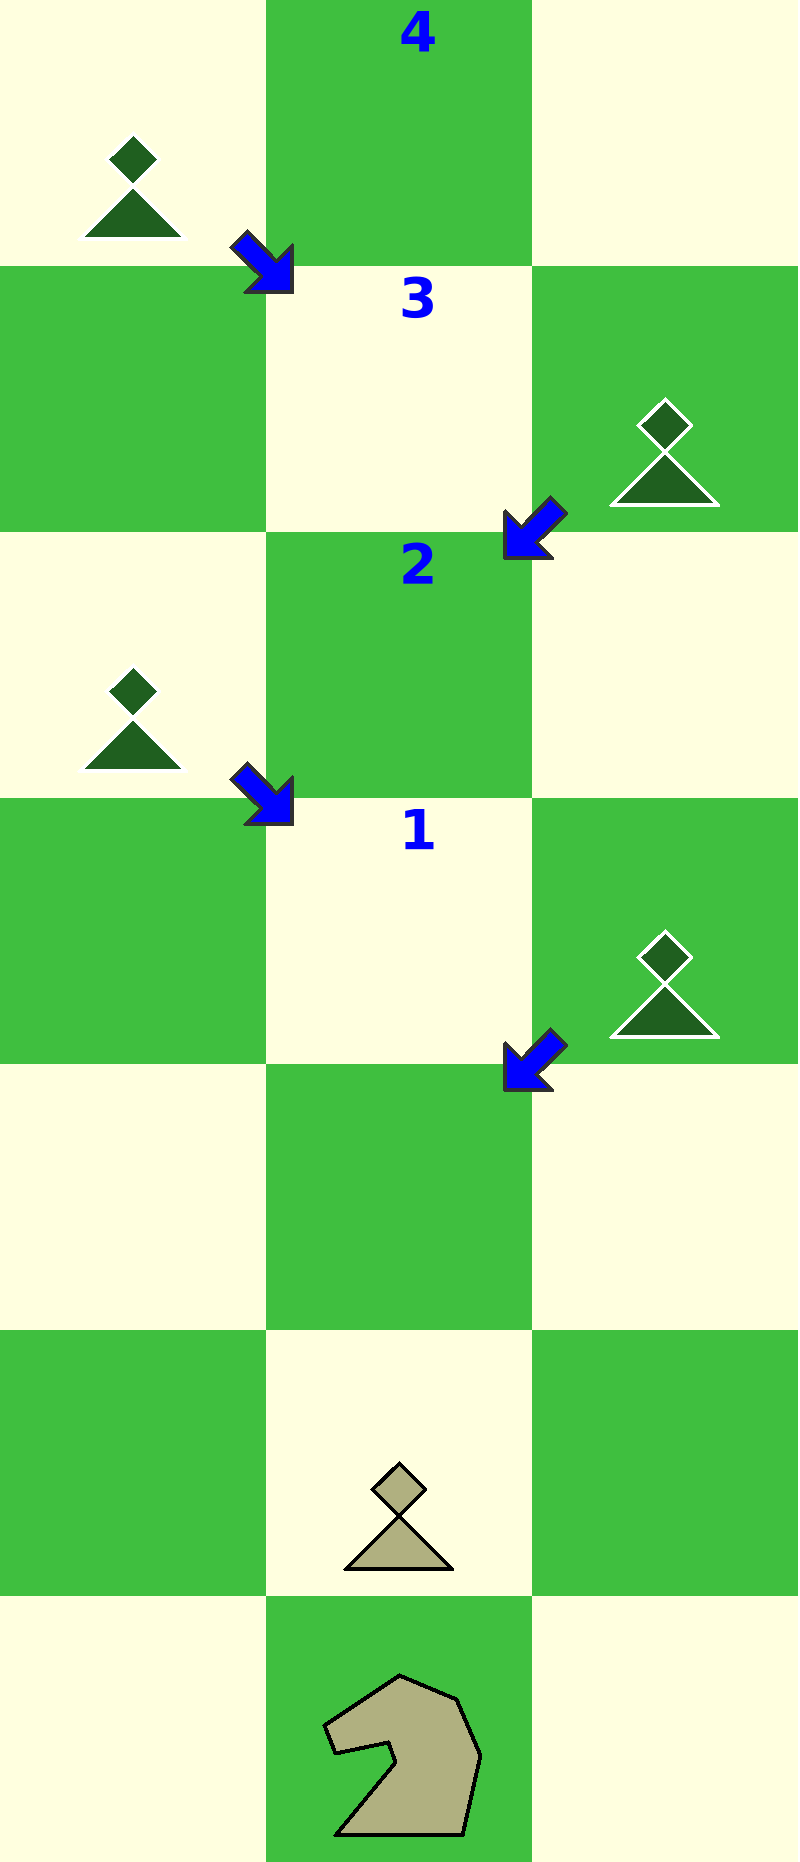
\includegraphics[width=0.214285714286\textwidth, keepaspectratio=true]{en_passants/08_age_of_aquarius_en_passant.png}
\caption{En passant}
\label{fig:08_age_of_aquarius_en_passant}
\end{wrapfigure}
Rush and en passant are identical to those in Classic Chess, only difference
is that Pawn can now move longer on initial turn, up to 5 fields in this
variant.

\clearpage % ..........................................................

\section*{Castling}
\addcontentsline{toc}{section}{Castling}

Castling is the same as in Classical Chess, only difference is that King can move 2, 3, 4 or 5 fields across.
All other constraints from Classical Chess still applies.

\noindent
\begin{figure}[!h]
% \begin{figure}[!t]
\includegraphics[width=1.0\textwidth, keepaspectratio=true]{castlings/08_aoa/age_of_aquarius_castling.png}
\caption{Castling}
\label{fig:age_of_aquarius_castling}
% \centering
\end{figure}

In example above, all valid King's castling moves are numbered.

\noindent
\begin{figure}[!h]
% \begin{figure}[!t]
\includegraphics[width=1.0\textwidth, keepaspectratio=true]{castlings/08_aoa/age_of_aquarius_castling_left_04.png}
\caption{Castling long left}
\label{fig:age_of_aquarius_castling_left_04}
% \centering
\end{figure}

In this example King was castling long to the left. Initial King's position is marked with "K".
After castling is finished, left Rook ends up on the field immediately right to the King.

\clearpage % ..........................................................

\section*{Initial setup}
\addcontentsline{toc}{section}{Initial setup}

Compared to initial setup of Mayan Ascendancy, Unicorn is inserted between Pyramid and Knight
symmetrically, on both sides of chessboard. This can be seen in the image below:

\noindent
% \begin{figure}[t]
\begin{figure}[h]
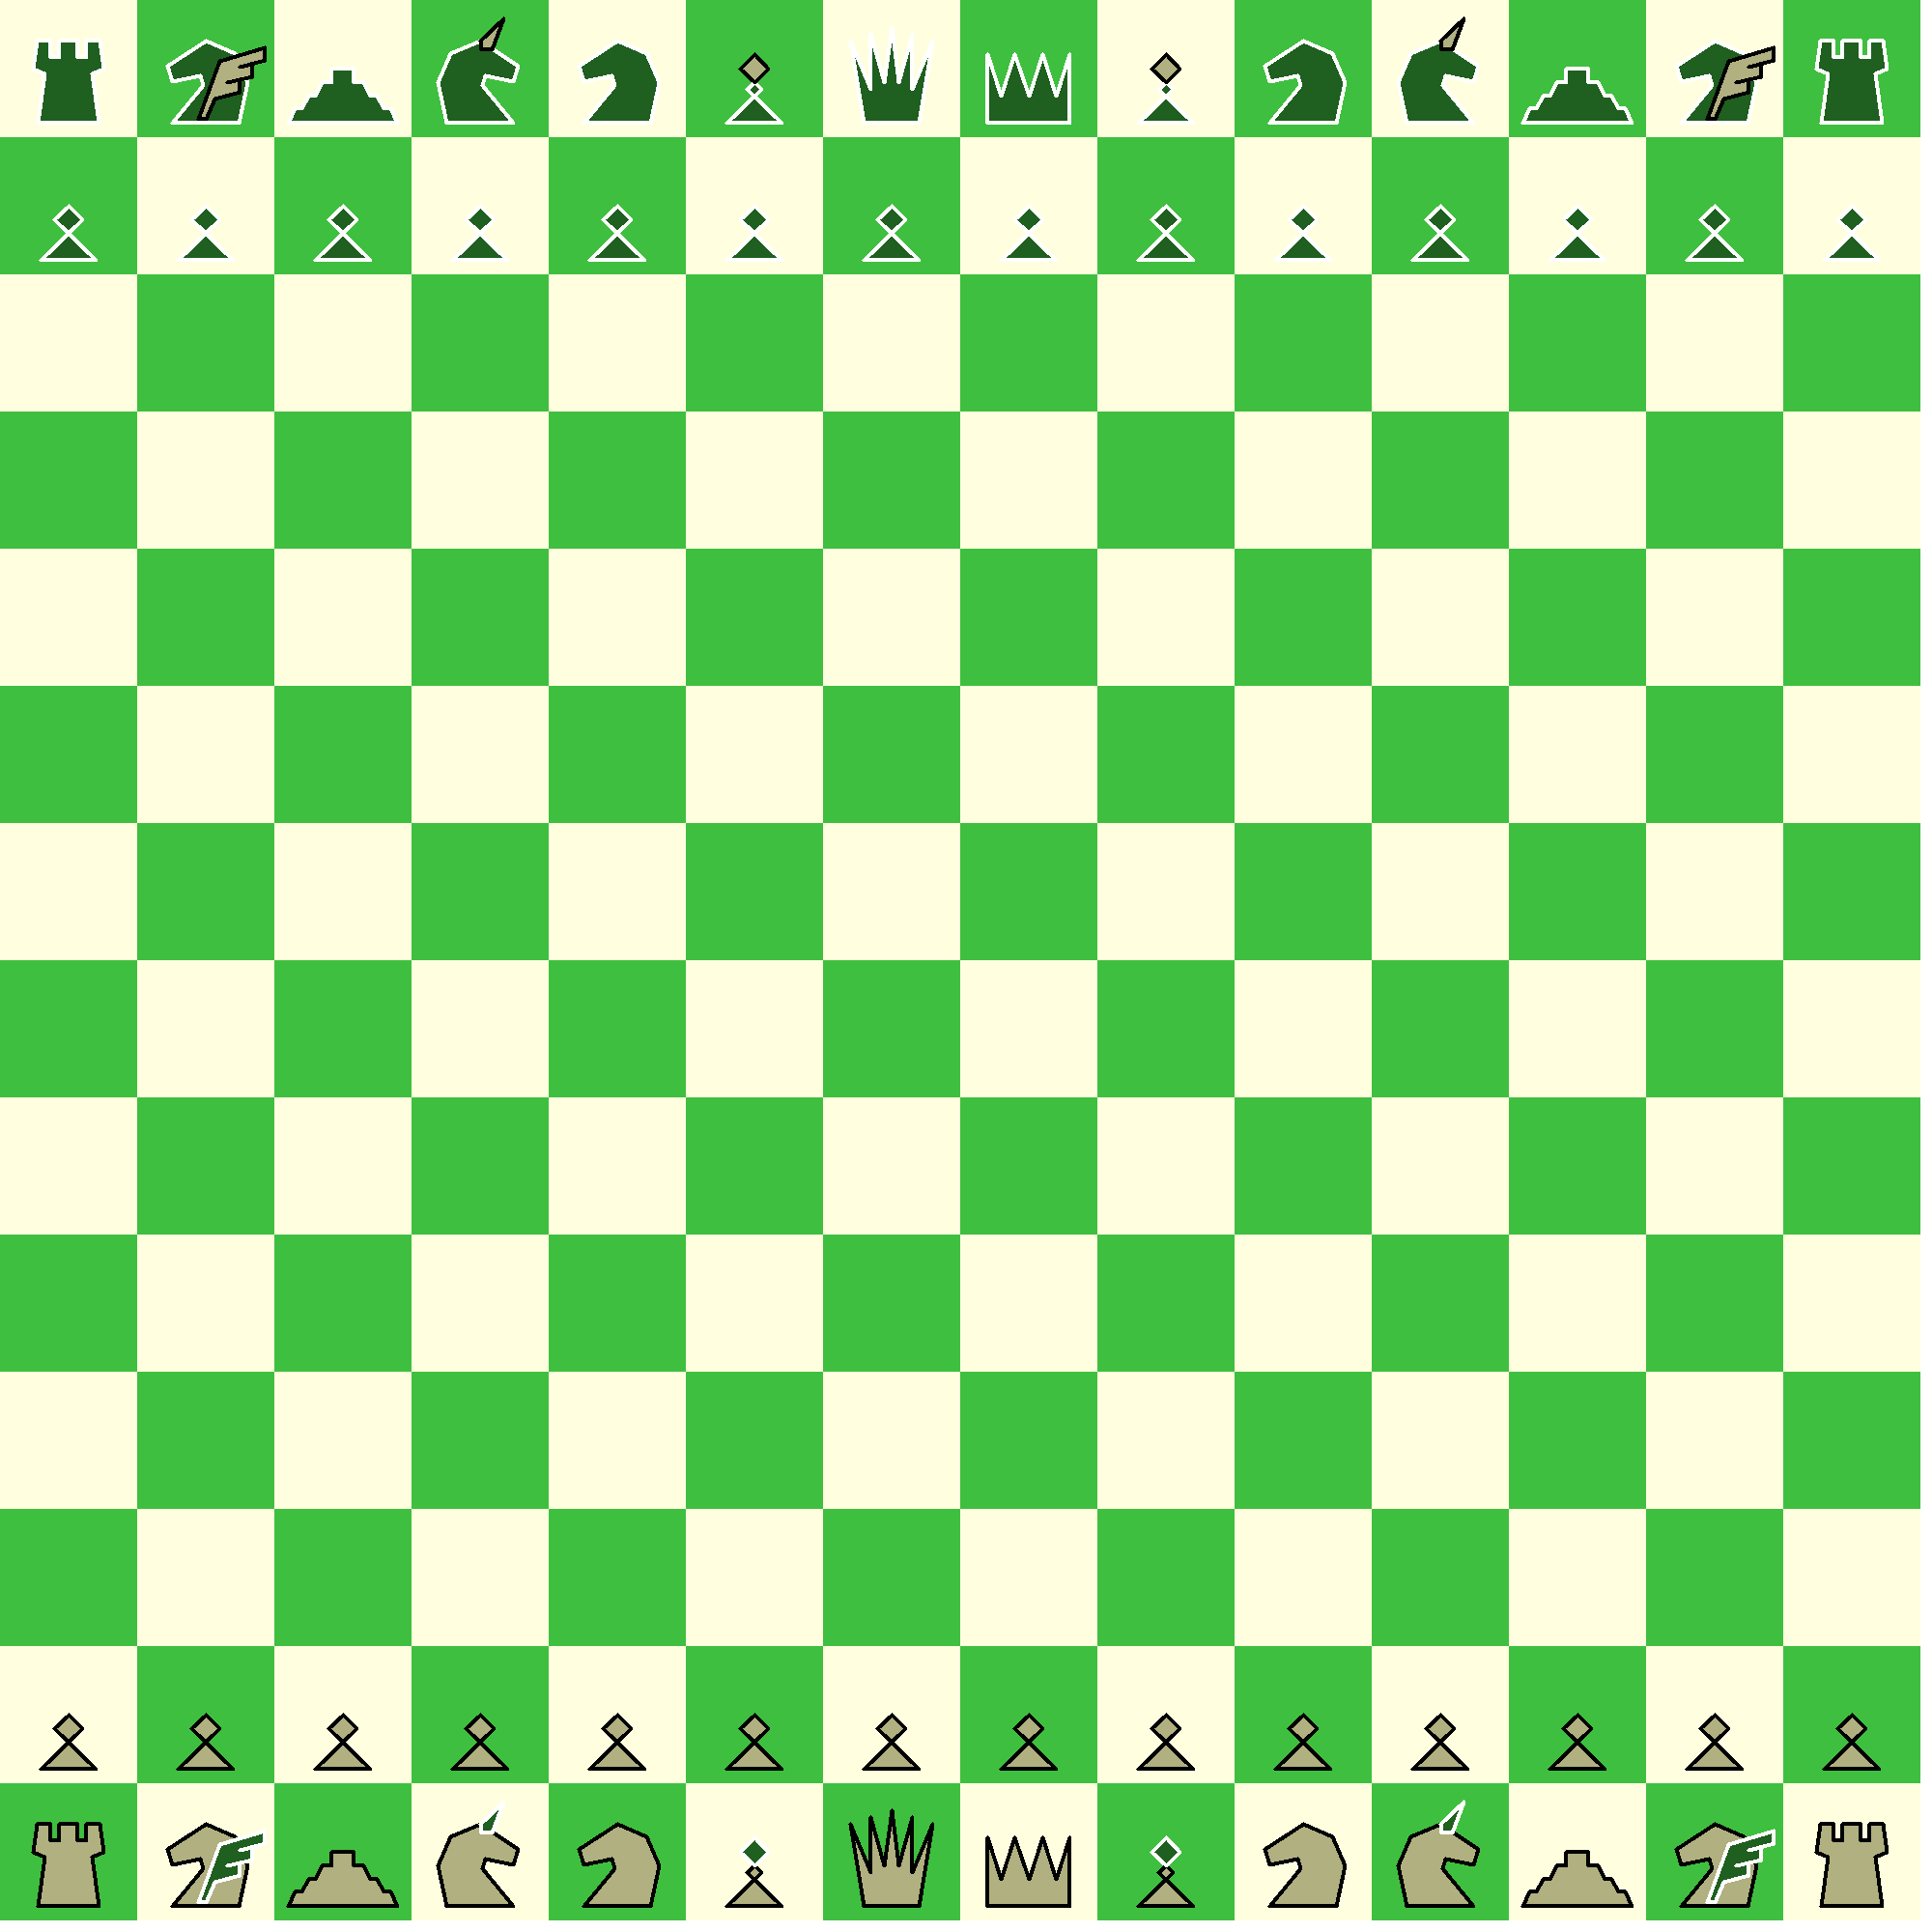
\includegraphics[width=1.0\textwidth, keepaspectratio=true]{boards/08_age_of_aquarius.png}
\caption{Age of Aquarius board}
\label{fig:08_age_of_aquarius}
% \centering
\end{figure}

\clearpage % ..........................................................
% ============================================= Age of Aquarius chapter
